\appendix
\chapter{Installazione e Configurazione del lato Server}

    In questa sezione vediamo in maniera molto rapida come siamo riusciti a 
    mettere in piedi il lato server per l'applicazione.
    
    
    \section{CouchDB}
        
        Come prima cosa dobbiamo tenere a mente che Apache 
        CouchDB\texttrademark{} non prevede la possibilità di gestire query 
        spaziali e per questo motivo sarà necessario installare l'estensione 
        Geocouch\footnote{Il repository GIT è reperibile all'indirizzo 
        \url{https://github.com/couchbase/geocouch/tree/couchdb1.3.x}}.
        
        Nel nostro caso abbiamo installato tutto il lato server 
        dell'applicazione su una macchina Arch Linux in quanto, per questo 
        sistema, era presente tra i suoi repository software ufficiali la 
        versione più aggiornata del DBMS (versione 1.5). Per installare Apache 
        CouchDB\texttrademark{} è stato sufficiente il comando:
        \begin{lstlisting}
    sudo pacman -S couchdb
        \end{lstlisting}
        
        Una volta terminata l'installazione abbiamo reso 
        il server raggiungibile dall'esterno modificando il file di 
        configurazione \texttt{/etc/couchdb/default.ini}: all'interno della 
        sezione \verb|[httpd]| abbiamo inserito l'indirizzo IP della macchina 
        come mostrato nel segmento del file seguente.
        \begin{lstlisting}
[...]
    keyvalue_buffer_size = 2097152 ; value in bytes
    [httpd]
    port = 5984
    bind_address = 192.168.0.5
    authentication_handlers = {couch_httpd_oauth,oauth_authentication_handler},{couch_httpd_auth,cookie_authentication_handler},{couch_httpd_auth, default_authentication_handler}
[...]
        \end{lstlisting}
        A questo punto, una volta riavviato il servizio, il server è 
        raggiungibile dall'esterno e può essere configurato comodamente dalla 
        propria interfaccia web che in questo caso è raggiungibile dall'url 
        \begin{lstlisting}
 http://192.168.0.5:5984/_utils/config.html
        \end{lstlisting}
        
        \noindent Adesso è necessario configurare:
        \begin{description}
            \item[cors] in modo che il server accetti messaggi \html{} 
            particolari provenienti da un dominio differente da quello locale. 
            In particolare, all'interno della sezione \texttt{cors}, bisogna 
            settare i seguenti parametri:
            \begin{description}
                \item[credentials] va impostato a \texttt{true} in modo che il 
                server controlli le credenziali di accesso allegate al 
                messaggio HTTP che riceve;
                \item[headers] deve contenere l'elenco degli header HTTP che 
                vogliamo siano accettati che nel nostro caso sono: 
                \texttt{accept}, \texttt{authorization},\\
                \texttt{content-type}, \texttt{origin}, \texttt{x-titanium-id};
                \item[methods] devo contenere l'elenco dei metodi HTTP che 
                vogliamo siano accettati e nel nostro caso sono: \texttt{HEAD}, 
                \texttt{GET}, \texttt{PUT}, \texttt{POST}, \texttt{DELETE};
                \item[origins] deve essere configurato in modo che vengano 
                accettate richieste HTTP provenienti da qualsiasi dominio, per 
                questo motivo abbiamo settato il valore ad \texttt{*}.
            \end{description}
            \item[couch\_httpd\_auth] in modo che vengano accettate solo richieste 
            provenienti da utenti registrati; in particolare i parametri da 
            configurare sono:
                \begin{description}
                    \item[require\_valid\_user] va impostato a \texttt{true} 
                    proprio per il suddetto motivo;
                    \item[public\_fields] va impostato con un elenco dei campi 
                    utente che vogliamo rendere pubblici; per la nostra 
                    applicazione avevamo la necessità di avere i campi 
                    \texttt{nick}, \texttt{mail} reperibili da qualsiasi altro utente;
                \end{description}
        \end{description}
        La configurazione completa è mostrata in fig. \ref{fig:confCouch1}.
        \begin{figure}[H]
            \centering
            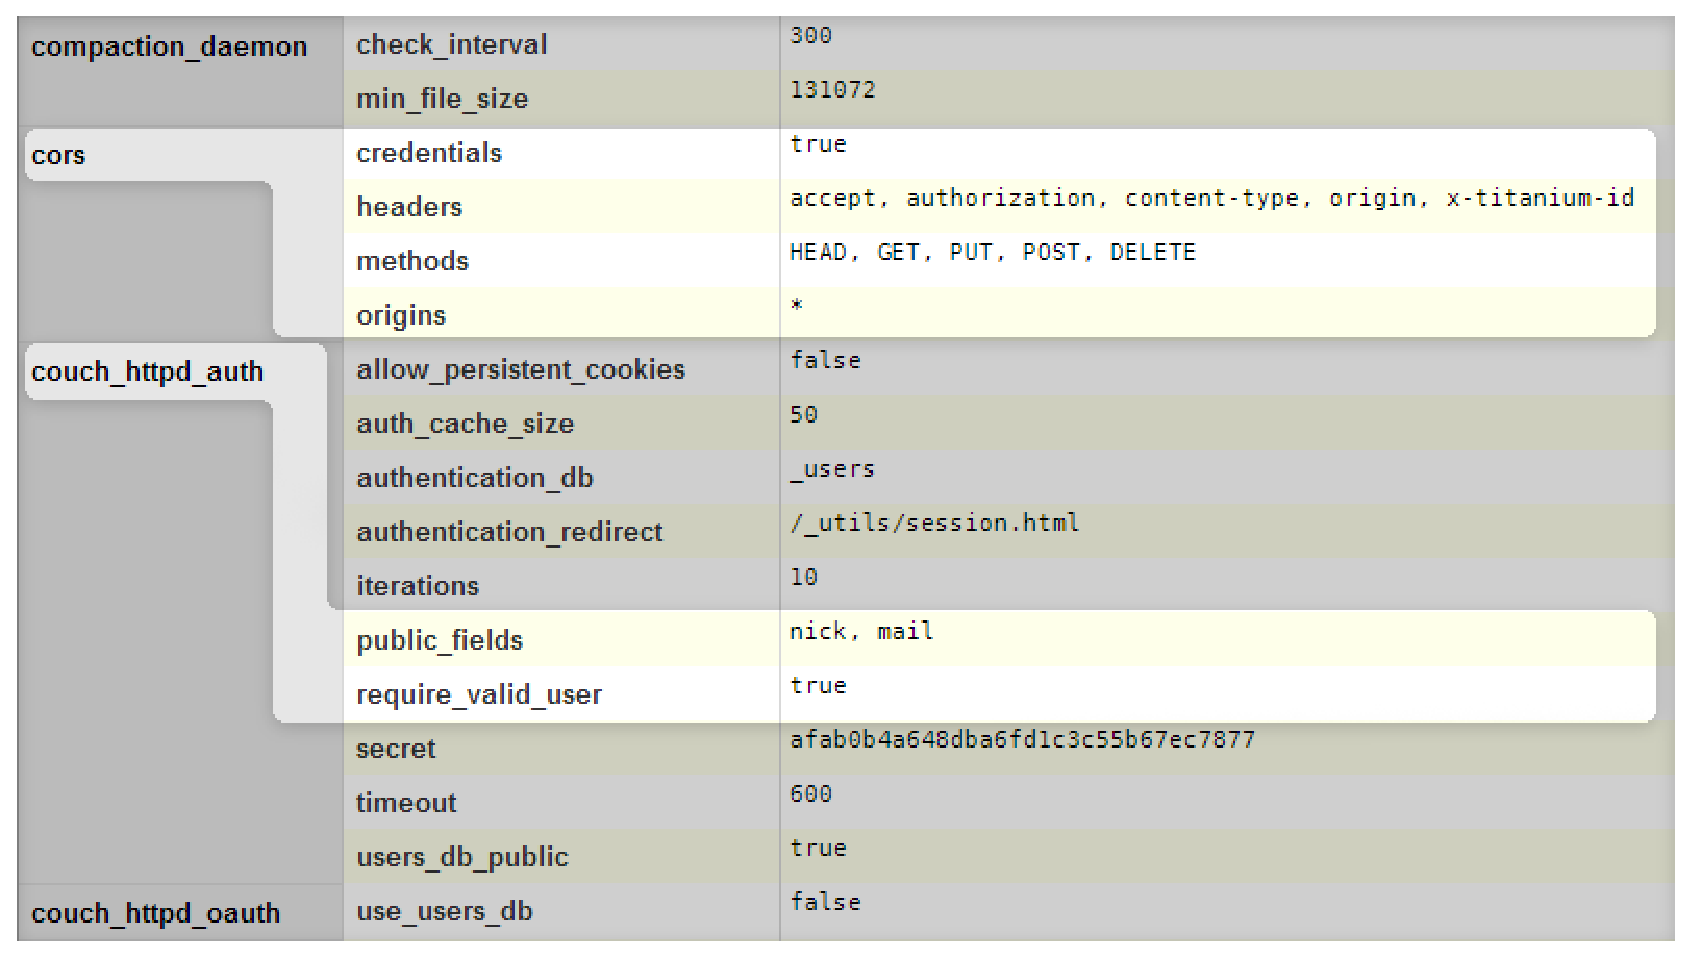
\includegraphics[keepaspectratio=true, width=0.99\textwidth]{couchConf1}
            \caption{
                Configurazione essenziale per rendere possibile la comunicazione
                della app con il server.
            }
            \label{fig:confCouch1}
        \end{figure}

        \subsection{Geocouch}
            Una volta che Apache CouchBD\texttrademark{} è stato installato e 
            configurato abbiamo provveduto ad installare l'estensione per 
            poter effettuare query spaziali sulle coordinate geografiche 
            associate ad ogni segnalazione.
            
            Geocouch non è presente tra i repository standard di Arch Linux ma 
            è disponibile in AUR (Arch User Repository)\footnote{Una guida 
            completa su come utilizzare questo repository è disponibile 
            all'url 
            \url{https://wiki.archlinux.org/index.php/Arch_User_Repository_(Italiano)}.}
            così anche in questo caso siamo riusciti ad installare tutto con 
            pochi semplici comandi:
            \begin{description}
                \item[ottenere il tarball]
                Prima di tutto è necessario recuperare il pacchetto 
                contenente i sorgenti reperibile all'indirizzo 
                \url{https://aur.archlinux.org/packages/ge/geocouch/geocouch.tar.gz}.
                \item[estrarre il pacchetto]
                Estrarre il tarball (preferibilmente in una cartella da tenere 
                da parte solo per le compilazioni di AUR) con il comando
                \begin{lstlisting}
    tar -xzf geocouch.tar.gz
                \end{lstlisting}
                \item[compilare il pacchetto installabile]
                Lanciare il comando \texttt{makepkg} all'interno della directory
                contenente i file scaricati (il comando \texttt{makepkg -s} si 
                occuperà di risolvere automaticamente le dipendenze tramite 
                pacman). Questo scaricherà e compilerà il codice, infine 
                creerà il pacchetto.
                \begin{lstlisting}
    cd geocouch/
    makepkg -s
                \end{lstlisting}
                \item[Intallare Geocouch]
                Installare il pacchetto ottenuto tramite \texttt{pacman}:
                \begin{lstlisting}
    sudo pacman -U geocouch-1.3.1-1-armv6h.pkg.tar.xz
                \end{lstlisting}
            \end{description}
            Terminata l'installazione è sufficiente un riavvio del servizio 
            CouchDB per rendere operativa l'estensione installata.
